\section{The System's Components Design}
\subsection{Purpose of Component Diagram}

Component diagrams allow stakeholders and development staff to appreciate the role of modular parts of a software application and to ensure reliability and extensibility. This causes improvements in software delivery times, development costs and quality\cite{felicicomp}.

The components are the physical and replaceable building blocks of software systems, whereas the interface describes a group of operations used or created by components\cite{microsoftcomp}. There are also ports, which are explicit windows into an encapsulated component and parts which are units of the implementation of the component. The component diagram model has visual representations of the components and how they connect between each other\cite{bellcomp}.

\begin{figure}[H]
    \centering
    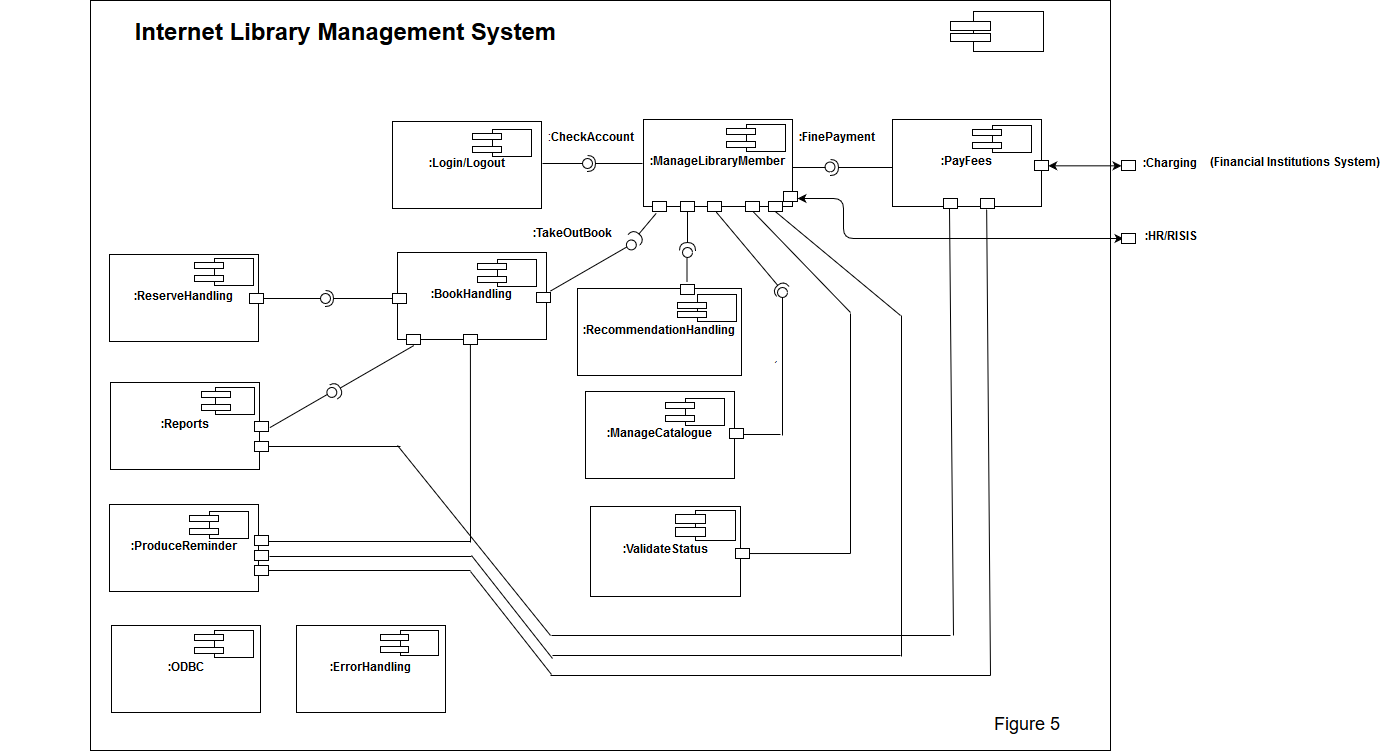
\includegraphics[width=\linewidth]{image/component.png}
    \caption{Component Diagram}
    \label{fig:component}
\end{figure}

The first component Login/Logout will handle all logging in and logging out functions. It checks credentials and allows the general public to register. This will also handle errors such as incorrect logins and forgotten passwords. This has an interface connection to ManageLibraryMember, which handles everything regarding the library user and what they can do with their library membership. There is another interface connection to PayFees which has an external connection to a banking system. This allows library members to handle any outstanding fines that they have to pay. ManageLibraryMember also has an external connection to HR/RISIS, which allows the external employers to manage fines and reports for each library member. ManageLibraryMember has an interface connection to RecommendationHandling, which handles the recommendations that specific users can do. ManageCatalogue has an interface connection to ManageLibraryMember which manages the inventory of the library. This includes functions such as update catalogue. There is a direct connector between ManageLibraryMember and ValidateStatus where ValidateStatus handles specific validation. BookHandling has an interface connection to ManageLibraryMember. BookHandling handles all the functions regarding the books. This includes functions such as take out book and return book. It also has an interface connection to ReserveHandling, since books can be reserved and each book will need a handling component for this. BookHandling also has an interface connection to Reports, since when handling members who have taken out books, reports must also be generated for that specific book if it is not returned. BookHandling has a direct connector to ProduceReminder, which produces reminders for the specific book that members have taken out or reserved. Finally ManageLibraryMember has a direct connection to ProduceReminder, since reminders (book overdue, fine overdue, membership due, book available) need to be produced for members who are using the library. PayFees has a direct connection to Reports and ProduceReminders. Reminders and reports will always be produced for members who will need to pay some sort of fees. The ODBC (Open Database Connectivity) and ErrorHandling will be used by the ILMS as a whole and so are the individual components.
